% Chapter 1
\definecolor{pink}{rgb}{1.0,.01,0.57}
\chapter{Frequency modulation} % Main chapter title
\label{Chapter2} % For referencing the chapter elsewhere, use \ref{Chapter1} 
\lhead{Chapter 2. \emph{Frequency modulation}} % This is for the header on each page - perhaps a shortened title
\textsf{\textsl{Written by Bjorn Deraeve}}
%----------------------------------------------------------------------------------------

\section{Introduction}
Thanks to new digital technology there was room for a new synthesis technique, Frequency Modulation Synthesis. The advantage of FM is that a very large number of different sounds can be produced with few elemental units (oscillators). In other words the timbral space is very large. The one requirement is the use of optimized computers, which is discussed in chapter \ref{Chapter5}.
%----------------------------------------------------------------------------------------

\subsection{Basic concepts of modulation synthesis}
It is important to know that in the synthesizer only one wave form, a sine wave, is stored. The trick of modulation synthesis is to remodel this wave until a desired sound is found. \\ An easy example is the square wave. Using additive synthesis a square wave can be built out of an infinite amount of sine functions. This example of additive synthesis also explains the Fourier transformation theory and is shown in figure \ref{fig:additive}.
\begin{figure}[ht]
  \hfill
  \begin{minipage}[t]{.45\textwidth}
    \begin{center}  
      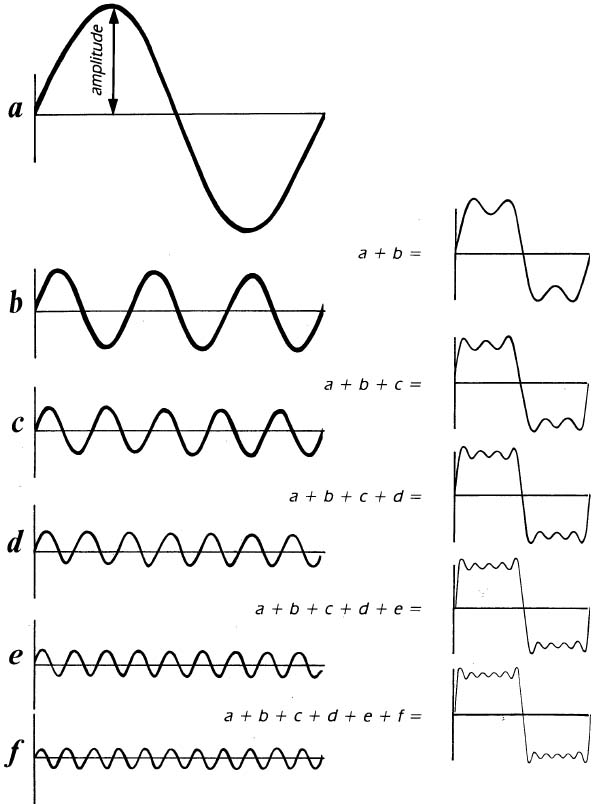
\epsfig{file=additive, scale=0.22}
      \caption{Additive synthesis of a square wave}
      \label{fig:additive}
    \end{center}
  \end{minipage}
  \hfill
  \begin{minipage}[t]{.45\textwidth}
    \begin{center}  
      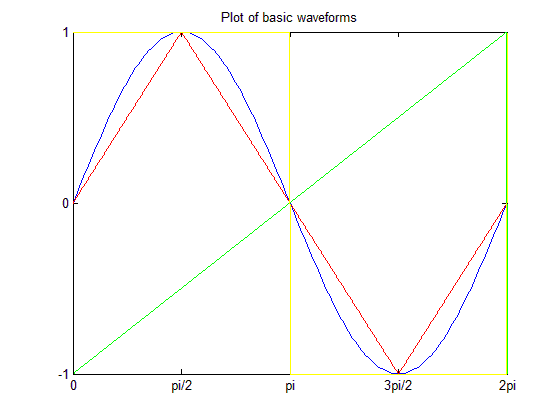
\epsfig{file=basicWaveforms.png, scale=0.33}
      \caption{Basic waveforms}
      \label{fig:basicWaveforms}
    \end{center}
  \end{minipage}
  \hfill
\end{figure}
%----------------------------------------------------------------------------------------
\subsection{Oscillators and operators}
The basic building blocks of FM synthesizers are operators. They are equivalent to oscillators in analogue synthesizers and produce the waveforms the user desires. Where an analogue oscillator produces a changing voltage the digital operator creates discrete samples according to a sine pattern. The operators invite the user to be creative in creating their own unique sound with the aid of different kinds of modulation techniques and waveforms. Knowing that most intersting sounds have many components, with the use of only four operators and modulation techniques one can generate sounds with much more than four partials.
\subsection{Waveforms}
To produce creative sounds it can be appropriate to combine sine waves with other waveforms. Synthesizers are typically able to produce sines, triangles, sawtooths and square waves.
A square wave contains only odd-integer harmonic frequencies. To be an ideal wave, the signal should change from high to low instanaeously. However this is impossible to achieve in real-world systems because of the limited bandwith, though good approximations can be made with additive synthesis. The Fourier series of the square wave is given in equation \ref{eq:square} \\
\begin{equation}
x(t) = \frac{4}{\pi} \sum_{n=1,3,5,...}^{\infty} \frac{\mathrm{sin}(2\pi \cdot n \cdot f \cdot t)}{n}
\label{eq:square}
\end{equation}
\begin{equation}
x(t) = \frac{4}{\pi} \Bigl( \mathrm{sin}(\omega t) + \frac{1}{3} \mathrm{sin} (\mathrm{3} \omega t) + \frac{1}{5}\mathrm{sin}(\mathrm{10}\omega t) + ... \Bigr)
\label{eq:square2}
\end{equation}
Triangle waves contain just like square waves only odd harmonics of the pitch. The difference is that the higher harmonics lose their energy faster. Equation \ref{eq:triangle} gives the Fourier series to approximate a triangle wave using additional synthesis.
\begin{equation}
x(t) = \frac{8}{\pi^{2}} \sum_{n=1,3,5,...}^{\infty} (-1)^{(n-1)/2} \frac{\mathrm{sin}(2\pi \cdot n \cdot f \cdot t)}{n^{2}}
\label{eq:triangle}
\end{equation}
\begin{equation}
x(t) = \frac{8}{\pi^{2}} \Bigl( \mathrm{sin}(\omega t) - \frac{1}{9} \mathrm{sin} (\mathrm{3} \omega t) + \frac{1}{25}\mathrm{sin}(\mathrm{5}\omega t) - ... \Bigr)
\label{eq:triangle2}
\end{equation} 
Finally sawtooth waves contain both even and odd harmonics of the fundamental frequency. The sound of it is even more raw. The equation for additive synthesis is given by equation \ref{eq:saw}.
\begin{equation}
x(t) = \frac{2}{\pi} \sum_{n=1}^{\infty} (-1)^{n+1} \frac{\mathrm{sin}(2\pi \cdot n \cdot f \cdot t)}{n}
\label{eq:saw}
\end{equation} 
\begin{equation}
x(t) = \frac{2}{\pi} \Bigl( \mathrm{sin}(\omega t) - \frac{1}{2} \mathrm{sin}(2\omega t) + \frac{1}{3} \mathrm{sin}(3\omega t) - ... \Bigr)
\label{eq:saw2}
\end{equation} 
\begin{figure}[htbp]
\centering
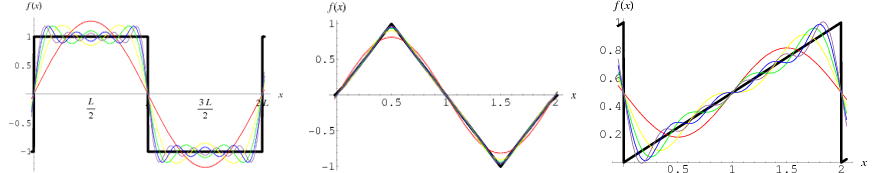
\includegraphics[height=3cm]{waves.png}
\rule{30em}{0.5pt}
\caption{Square, triangular and sawtooth wave synthesis}
\label{fig:waves}
\end{figure} \\
Figures \ref{fig:freqsquare}, \ref{fig:freqTriangle} and \ref{fig:freqSawtooth} show the corresponding frequency responses of the square, triangle and sawtooth wave and confirm equations \ref{eq:square}, \ref{eq:triangle} and \ref{eq:saw}. 
\begin{figure}[ht]
  \hfill
  \begin{minipage}[t]{.45\textwidth}
    \begin{center}  
      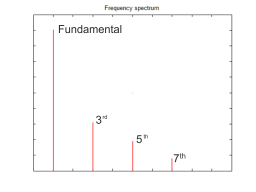
\epsfig{file=freqSquare.png, scale=0.30}
      \caption{Frequency spectrum of square wave}
      \label{fig:freqsquare}
    \end{center}
  \end{minipage}
  \hfill
  \begin{minipage}[t]{.45\textwidth}
    \begin{center}  
      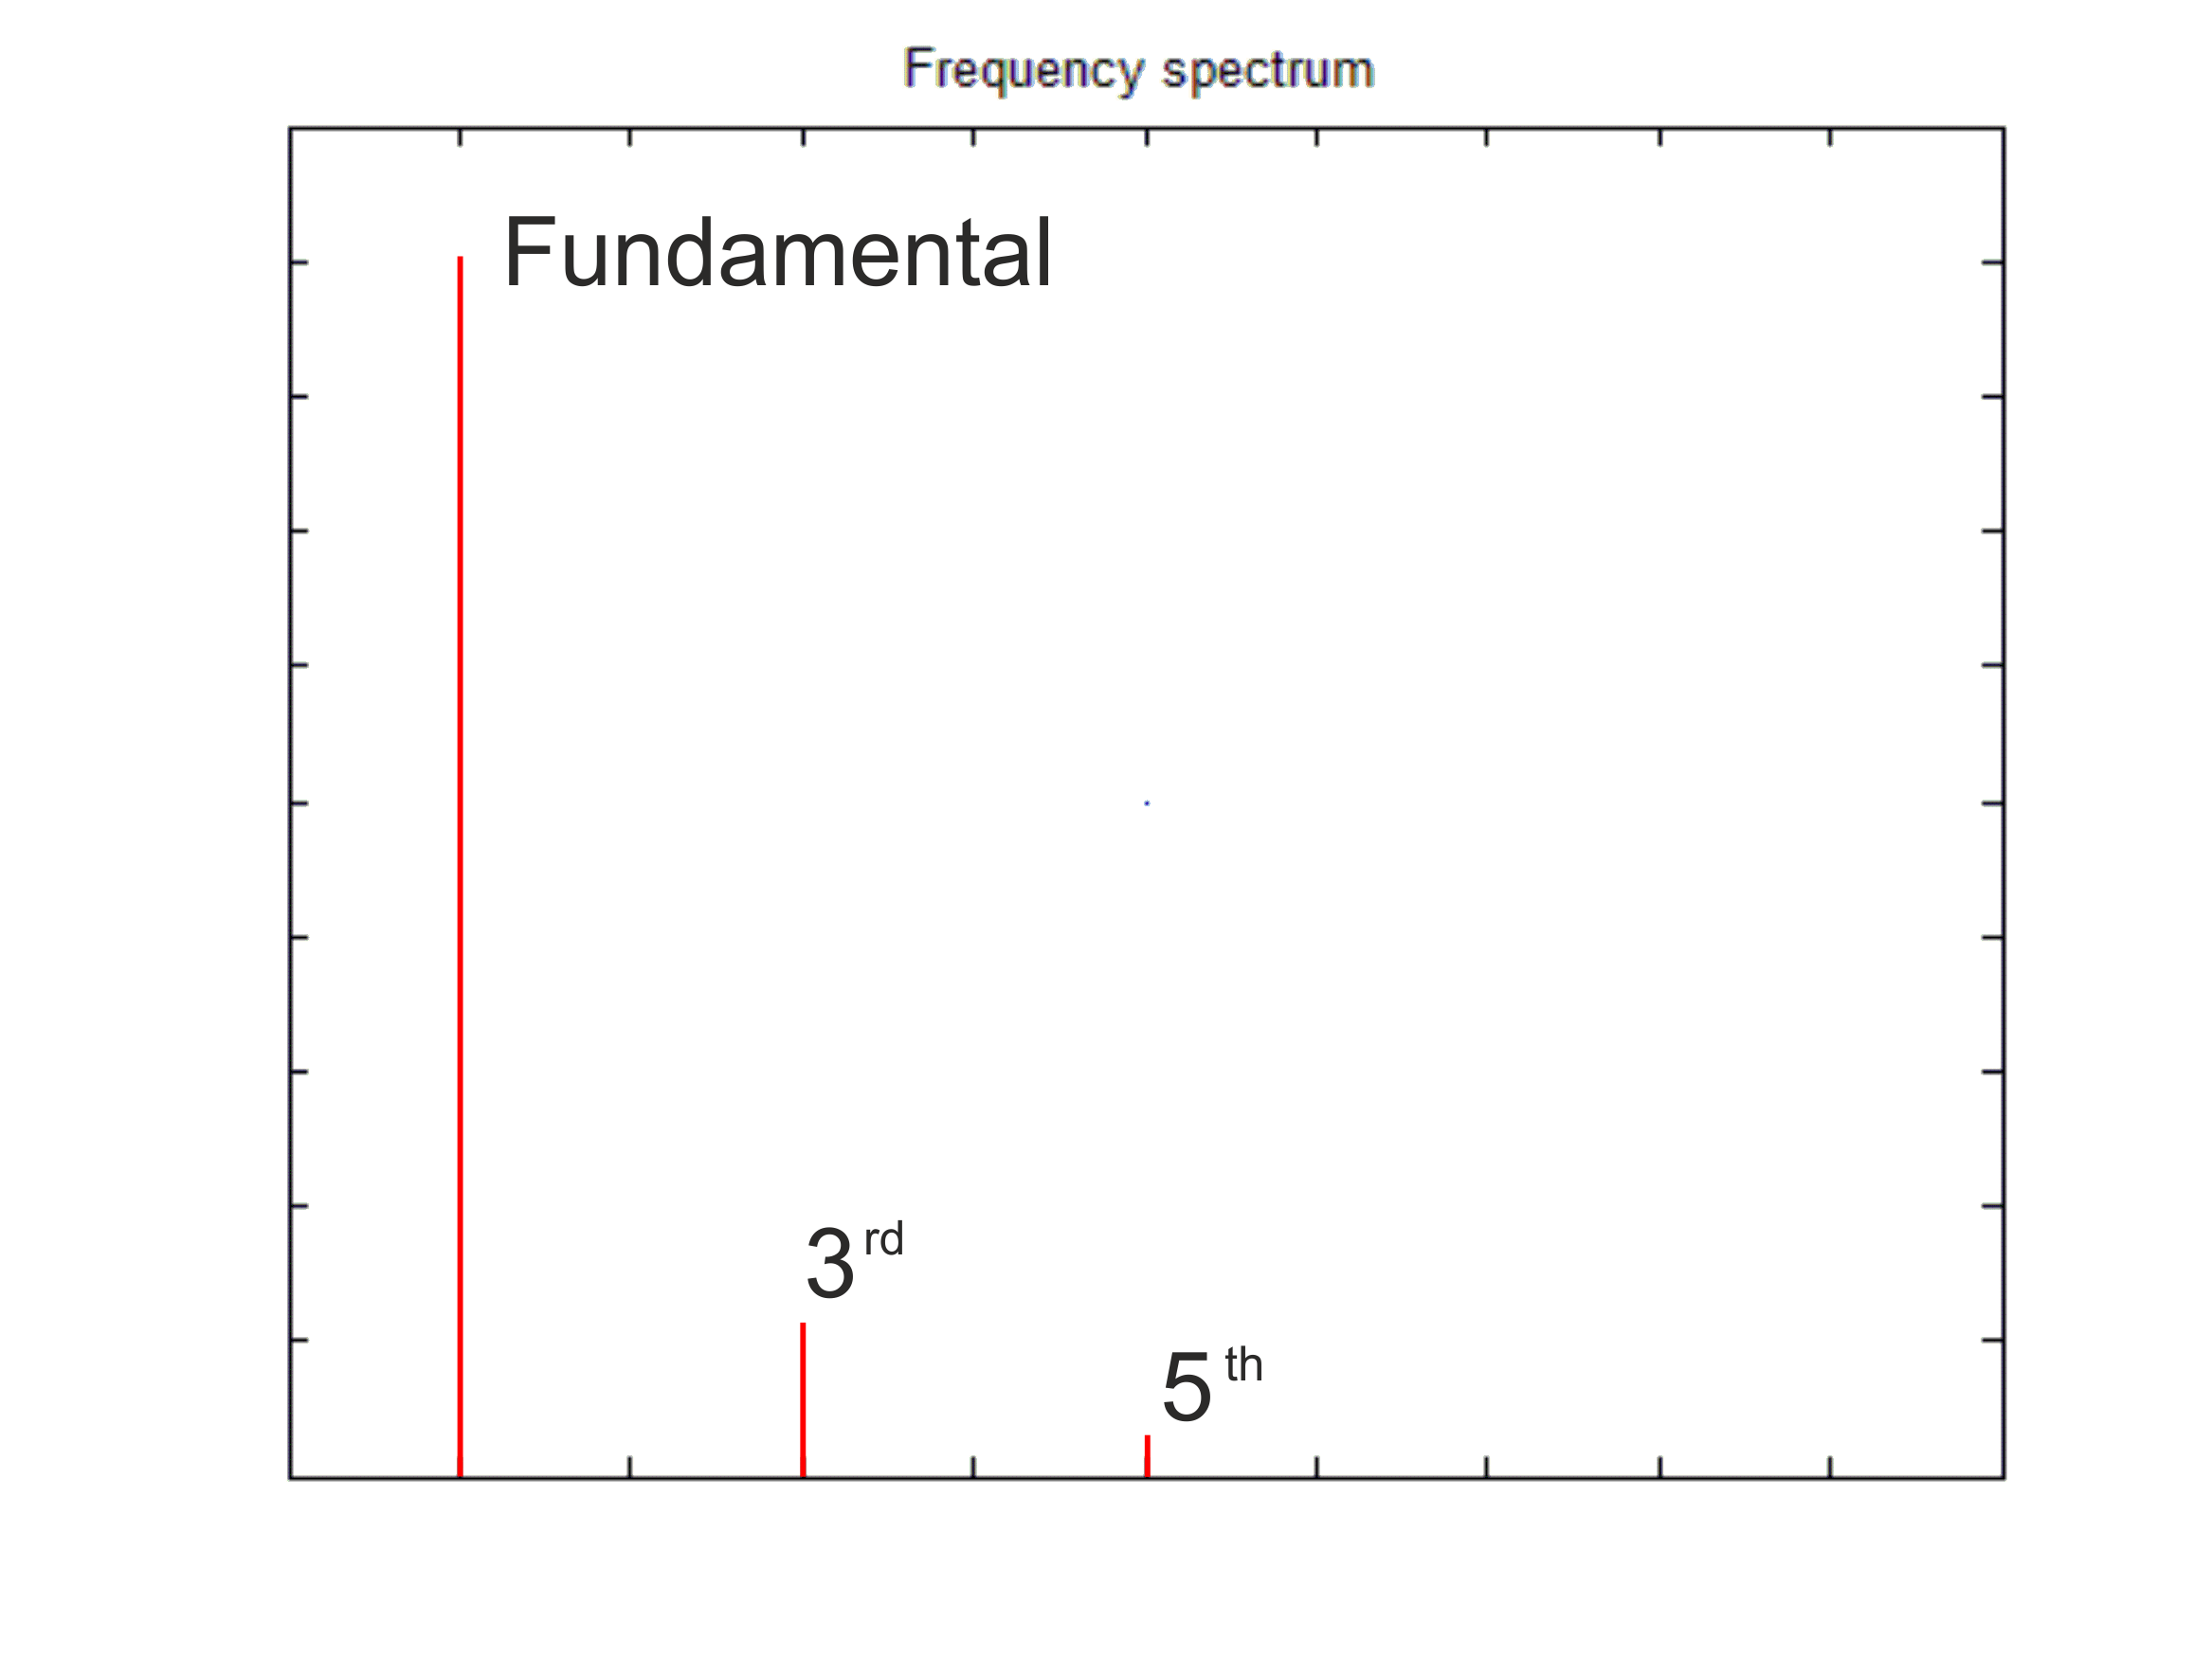
\epsfig{file=freqTriangle.png, scale=0.30}
      \caption{Frequency spectrum of triangular wave}
      \label{fig:freqTriangle}
    \end{center}
  \end{minipage}
  \hfill
\end{figure}
\begin{figure}[htbp]
\centering
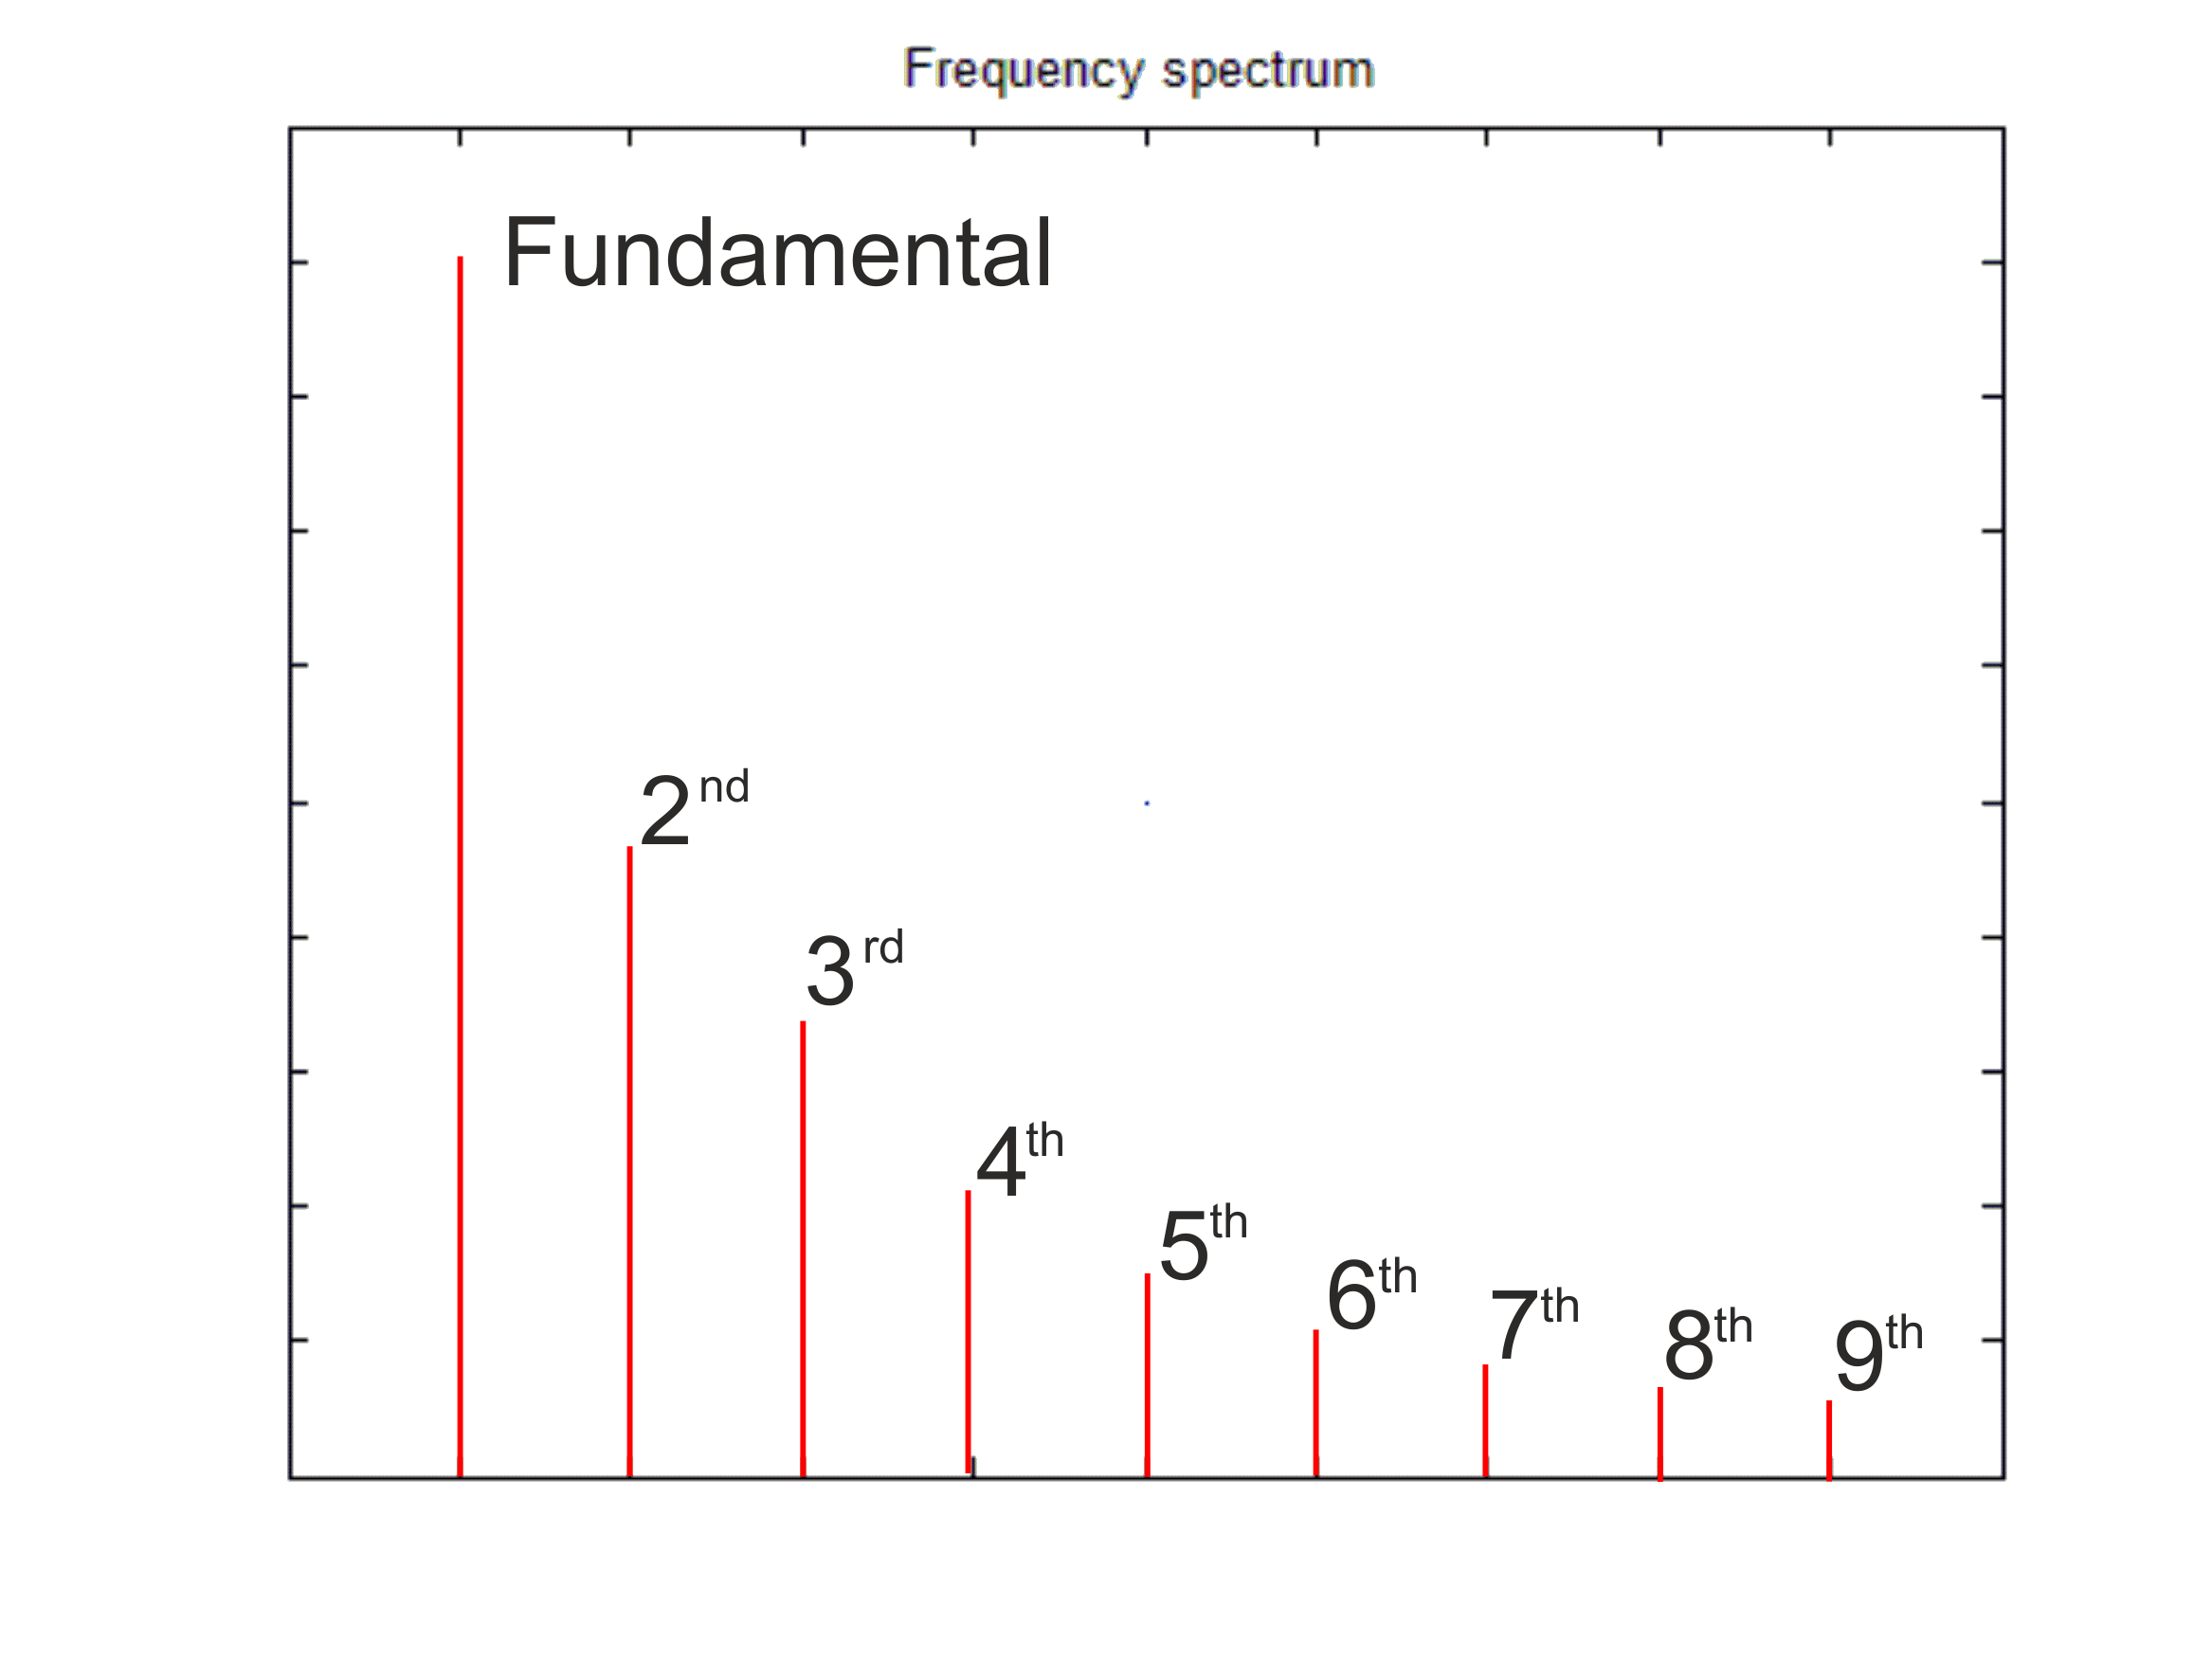
\includegraphics[height=4.8cm]{freqSaw.png}
\rule{30em}{0.5pt}
\caption{Frequency spectrum of sawtooth wave}
\label{fig:freqSawtooth}
\end{figure}
%----------------------------------------------------------------------------------------
\section{Mathematical approach}
The most basic form of frequency modulation is vibrato, in fact, FM is simply very fast vibrato. This possibility to create completely new sounds has been discovered by John Chowning at Stanford University in the mid-'60s. He found that when the frequency of the modulator increases beyond a certain point, the vibrato effect is replaced by a complex new tone. \\
We can create a vibrato sound by letting operator 2 cause a small change in frequency of operator 1. The rate and amount of frequency change is determined by operator 2. When the waveform of operator 2 increases the tone becomes brighter. This means that more harmonics are appearing in the frequency spectrum. Referring to the introduction section of this chapter, we remark again that FM is able to produce a wide variety of interesting spectra with only two basic oscillators. \\

Equations \ref{eq:sina} and \ref{eq:sinb} are two basic sines. The instantaneous amplitude of the waves at any given point in time is called 'A' and are related to their gains 'a' (maximum amplitude of their cycle).
\begin{equation}
\mathrm{A_{c}(t) = a_{c}\,sin(2\pi f_{c} t)}
\label{eq:sina}
\end{equation}
\begin{equation}
\mathrm{A_{m}(t) = a_{m}\,sin(2\pi f_{m} t)}
\label{eq:sinb}
\end{equation}\\
Equations \ref{eq:fma} and \ref{eq:fmb} define the frequency modulation of the carrier wave $A_{c}$(t) by the modulation wave $A_{m}$(t).
\begin{equation}
\mathrm{A_{c}(t) = a_{c}\,sin(\,(2\pi f_{c} + A_{m} )\, t)}
\label{eq:fma}
\end{equation}
\begin{equation}
\mathrm{A_{c}(t) = a_{c}\,sin(\,(2\pi f_{c} + a_{m}\,\mathrm{sin}(2\pi f_{m} t ))\, t)}
\label{eq:fmb}
\end{equation}
Looking at equation \ref{eq:fmb} we see the modulated signal consists of a constant amplitude $a_{c}$ and a time varrying argument to the sine function, or phase function $\phi$(t). This phase function is the addition of a constant ramp with slope 2 $\pi f_{c}$ and a sinusoidal variation, see picture \ref{fig:phasefunction}.
\begin{figure}[htbp]
\centering
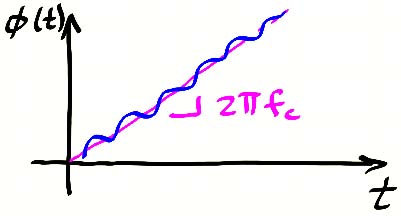
\includegraphics[height=3.5cm]{phasefunction}
\rule{30em}{0.5pt}
\caption{Phase function}
\label{fig:phasefunction}
\end{figure}
The phase function has two parameters that influence the nature of the modulated signal: $a_{m}$ and $f_{m}$. The degree to which this variation is added to the constant ramp is given by the modulation index $a_{m}$ or also referred to as I. So the modulation index describes the amount of frequency deviation. $f_{m}$ is the modulation frequency and defines the rate at which the frequency deviation is to occur.\\ Now how does this influence the sound of a frequency modulated signal? First one must see that the side bands produced by FM lie around the carrier frequency, being plus or minus an integer multiple of the \emph{modulator frequency} (the 1$^{st}$ parameter of $\phi$(t)). This is expressed by equation \ref{eq:sidebands} and visible in figure \ref{fig:sidebands}.
\begin{equation}
\mathrm{f_{sb} = 2\pi f_{c} \pm \mathrm{n} \cdot 2\pi f_{m} }
\label{eq:sidebands}
\end{equation}
\begin{figure}[htbp]
\centering
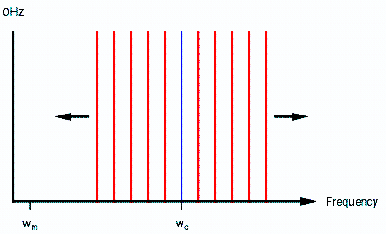
\includegraphics[height=3.5cm]{sidebands.png}
\rule{30em}{0.5pt}
\caption{The position of the side bands}
\label{fig:sidebands}
\end{figure}\\
The other parameter of the phase function is the \emph{amplitude of the modulator signal} and has a direct relation to the modulation index I. The modulation index  is defined as the ratio of the change in carrier frequency to the modulator frequency:
\begin{equation}
\mathrm{I = \frac{ \Delta \omega_{c} }{ \omega_{m} }}
\label{eq:I}
\end{equation}
Obviously the change in carrier frequency is determined by the amplitude of the modulator signal $a_{m}$. For any given modulator frequency, it is the modulation index (and thus the amplitude of the modulator) that defines the energy of each of the components in the spectrum. Also the height of the carrier frequency can be influenced by the value of I.\\ In fact the amplitude of the sidebands is controlled by a Bessel function $J_{k}$(a). Equation \ref{eq:fmb} can be rewritten as an infinite summation given by equation \ref{eq:spectrumBessel}, in which $\theta$ corresponds to 2$\pi f_{c}$, a corresponds to $a_{m}$ (strictly spoken I) and $\beta$ corresponds to 2$\pi f_{m}$:
\begin{equation}
\mathrm{sin}\,(\theta + \mathrm{a}\, \mathrm{sin} \beta) = J_{0}(\mathrm{a})\,\mathrm{sin}\,\theta + \sum_{k=1}^{\infty} J_{k}(\mathrm{a}) \left[\,\mathrm{sin}\,(\theta + k\beta) + (-1)^{k}\mathrm{sin}\,(\theta - k\beta)\, \right]
\label{eq:spectrumBessel}
\end{equation}
In this equation sin($\theta$) corresponds to the component based on the carrier wave and the series of sin($\theta$ + k$\beta$) are for the side band components. Note that the amplitude of all the components is controlled by the Bessel functions.\\
First we will show exactly how the frequency of the modulator signal defines the position of the side band components: in equation \ref{eq:spectrumBessel} we see ''sin($\theta$)", this leads to the frequency component of the carrier \textcolor{blue}{$f_{c}$}, see picture \ref{fig:besselFreq}. If k equals one, the sine functions between brackets lead to frequency components of the modulator, \textcolor{pink}{$f_{c}$ + $f_{m}$} and \textcolor{pink}{$f_{c}$ - $f_{m}$}. If k equals two components \textcolor{red}{$f_{c}$ + 2$f_{m}$} and \textcolor{red}{$f_{c}$ + 2$f_{m}$} are formed. And so on. The effect of the negative components will be ignored from now on\footnote[1]{Since we deal with an infinite summation, the negative components will kind of mix into the positive components. This can be thought of as a kind of aliasing phenomenon.}.
\begin{figure}[htbp]
\centering
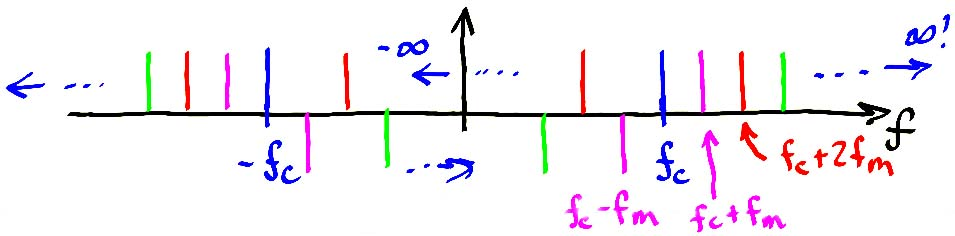
\includegraphics[height=2.1cm]{besselSpect}
\rule{30em}{0.5pt}
\caption{The position of the side bands}
\label{fig:besselFreq}
\end{figure}
Now we will have a look at how the Bessel functions control the amplitude of the side bands. Equation \ref{eq:bessel} defines a Bessel function with order $\alpha$.
\begin{equation}
x^{2} \frac{d^{2}y}{dx^{2}} + x\frac{dy}{dx} + (x^{2}-\alpha^{2})y = 0
\label{eq:bessel}
\end{equation}
As defined in equation \ref{eq:spectrumBessel}, the order of the Bessel function corresponds to the sideband number.  So figure \ref{fig:besselFunctions} shows 6 Bessel functions as a function of modulation index for a specific sideband number. \\
Note that, if the modulation index is zero (no modulation), the amplitude of the carrier frequency is equal to 1 (black curve). As we look at sidebands that are farther away from the carrier frequency we see that it takes longer for the amplitude of that sideband to become non-zero (\textcolor{red}{red}, \textcolor{blue}{blue},... curves). So one Bessel curve shows that the amplitude of the $n^{th}$ sideband depends on the modulation index. Or, for a given modulation index, the amplitude of the $n^{th}$ sideband is given by a Bessel function of order n.
\begin{figure}[htbp]
\centering
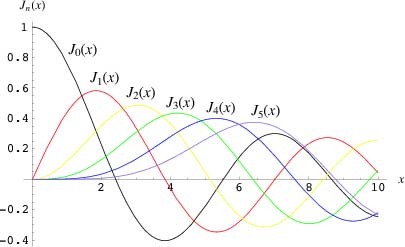
\includegraphics[height=4.9cm]{besselFunctions}
\rule{30em}{0.5pt}
\caption[Bessel functions for orders n = 0,1,2, $\cdots$]{Bessel functions for orders n = 0,1,2, $\cdots$. The order defines the curve, x-axis defines the modulation index and the y-axis returns the amplitude.}
\label{fig:besselFunctions}
\end{figure}\\
When the modulation index of the signals in figure \ref{fig:sidebands} is increased the spectrum will look like figure \ref{fig:sidebands2}:
\begin{figure}[htbp]
\centering
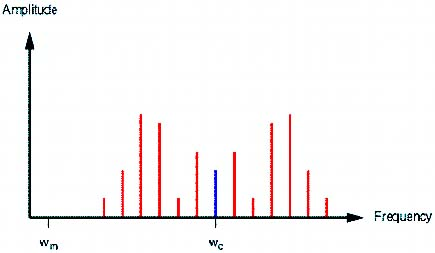
\includegraphics[height=4.0cm]{sidebands2}
\rule{30em}{0.5pt}
\caption{The amplitude of the sidebands.}
\label{fig:sidebands2}
\end{figure}\\
Appendix A contains a simple labview program to display Bessel functions of different orders and more examples that summarize this section.\\
%----------------------------------------------------------------------------------------
\section{Bandwidth considerations}
The bandwidth of the signal can be defined as the range of frequencies occupied by the signal. Allthough the sum series of sidebands is theoretically infinite, the modulation index will make sure that sidebands of higher frequency are very small and negligible.\\Equation \ref{eq:bw} gives an approximation of the bandwidth of a FM signal. 
\begin{equation}
B = 2\pi\,\mathrm{f_{m}} (1 +\mathrm{I}) 
\label{eq:bw}
\end{equation}
For example: the bandwidth of a signal with a 300Hz modulator with I = 5 will be 2 $\times$ 300Hz $\times$ (1+ 5) = 3600Hz. This show again that with FM it is easy to create complex signals with a much higher bandwidth.
%---------------------------------------------------------------------------------------- 
\section{Practical implementation}
Figure \ref{fig:funDesign} shows the practical implementation of the FM theory in our synthesizer program. In this figure the first modulation mode is shown where operator 2 modulates operator 1 according to formula \ref{eq:fmb}. The user can choose from this list of modulation types:
\begin{itemize}
\item 2 --$>$ 1
\item 3 --$>$ 2 --$>$ 1
\item 4 --$>$ 3 --$>$ 2 --$>$ 1
\item 4--$>$ 3 + 2 --$>$ 1
\end{itemize}
\begin{figure}[htbp]
\centering
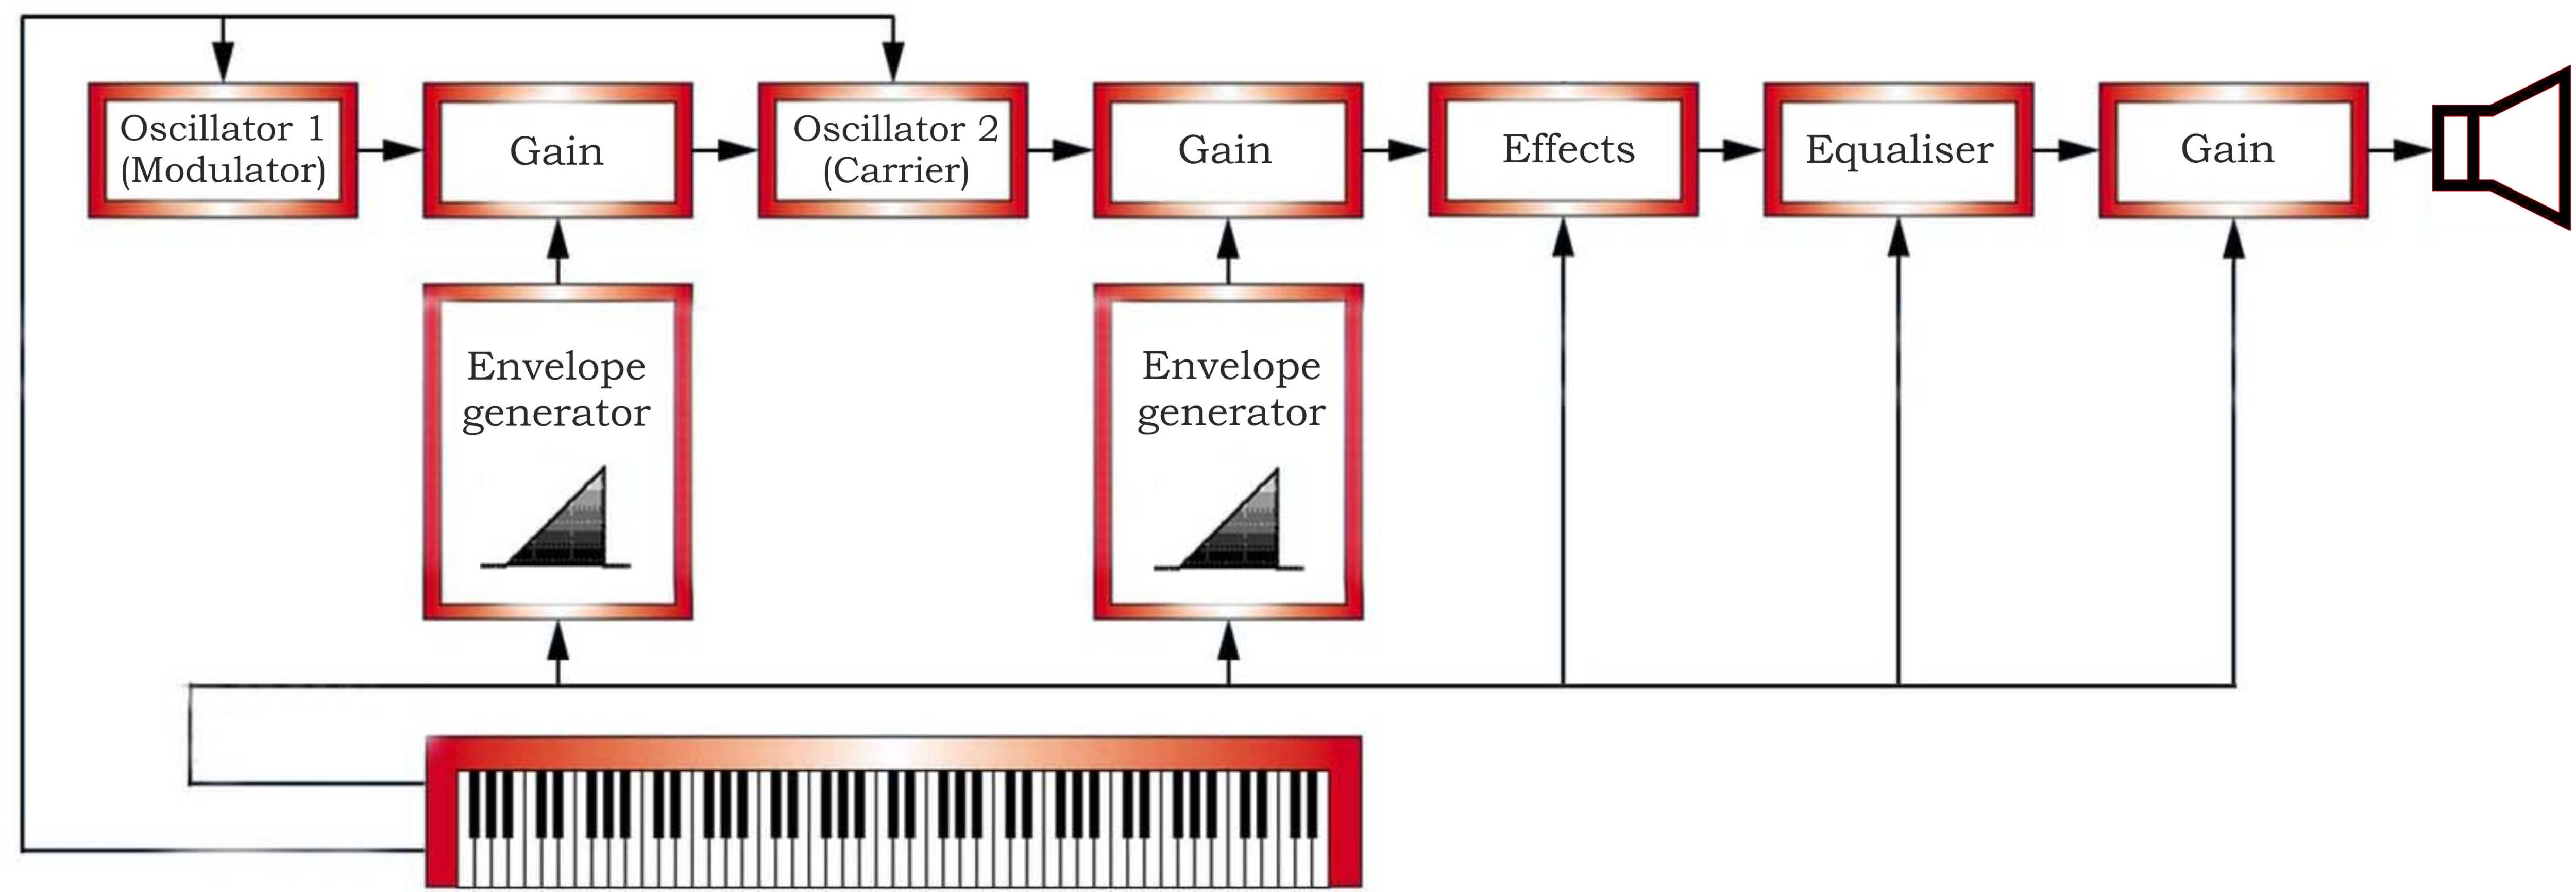
\includegraphics[height=5.0cm]{funDesign}
\rule{30em}{0.5pt}
\caption[Functional design of the FM synthesizer program]{Functional design of the FM synthesizer program \\ (First modulation type from the list above \\ (Compare this figure with the program flow chart \ref{fig:flowChart} discussed in chapter 6.)}
\label{fig:funDesign}
\end{figure}
For more information on the implementation of the FM synthesizer program please read chapters \ref{Chapter5}, \ref{Chapter7} and \ref{Chapter7}.\\ \\
\section{Summary}
%----------------------------------------------------------------------------------------
We've showed that frequency modulation is a very powerful method for music synthesis. It is possible to generate sounds that are not obtainable by any other modulation technique.\\
The carrier frequency sets the center of the sideband cluster, the modulator frequency only sets the sideband positions.\\
It is the modulation index that determines the amplitude of the sidebands and the number of significant sidebands, doing so shaping the spectrum.
